% don't remove the folling lines, and edit the defintion of \main if needed
\documentclass[../report.tex]{subfiles}
\providecommand{\main}{..}
\IfEq{\jobname}{\currfilebase}{\AtEndDocument{\biblio}}{}
% until here

%To have the commments written on the PDF: keep this macro
\newcommand{\commentsinout}[1]{#1}
%To have the commments hidden in the PDF: keep this macro
%\newcommand{\commentsinout}[1]{}

% this is a macro so you can make comments. See example below.
\newcommand{\KE}[1]{\commentsinout{{\bf{\color{brown} [KE: #1]}}}} % Comments by K. Ellis
\newcommand{\BH}[1]{\commentsinout{{\bf{\color{cyan} [BH: #1]}}}} % Comments by B. Heinemann
\newcommand{\FM}[1]{\commentsinout{{\bf{\color{orange} [FM: #1]}}}} % Comments by F. Maltoni
\newcommand{\AN}[1]{\commentsinout{{\bf{\color{teal} [AN: #1]}}}} % Comments by A. Nisati

\begin{document}
\linenumbers
\section{Introduction}

\subfile{\main/Neutrino/sub1/intro}


\subsection{The big questions related to the neutrino masses }

\subfile{\main/Neutrino/sub1/thintro}

\section{Present knowledge of neutrino mixing parameters}

\subfile{\main/Neutrino/sub1/PMNS}

\section{Measurements of neutrino oscillation parameters}
\subfile{\main/Neutrino/sub1/nuosc}
%\subsection{1.3.1 Running experiments (T2K, NOVA)}
%\subsection{ Future LBL experiments and sensitivity}
%(DUNE, HK, JUNO, ORCA)
%\subsection{ Precision flux and xsec measurements} (NA61, Near Detectors, Enubet,
%Nustorm)

%\section{  Measurements of neutrino mass and properties}
\subfile{\main/Neutrino/sub1/numass}
%(includes absolute mass, KATRIN, neutrinoless double beta searches, neutrino-
%nucleus coherent scattering)
\section{Search for new neutrino states}

An important question in neutrino physics is whether the 3-neutrino paradigm is complete or whether new neutrino states exist in nature. Their masses can range from the sub-eV scale up to the GUT scale. In the context of oscillation experiments eV to keV mass neutrinos are conventionally called sterile neutrinos, while heavier neutrino states with masses above MeV are often called Heavy Neutral Leptons (HNL).

\subsection{Searches for sterile neutrinos}
\subfile{\main/Neutrino/sub1/sterile}
\subsection{Searches for Heavy Neutral Leptons} \label{hnl-sec-nu}
\subfile{\main/Neutrino/sub1/hnl}

\subsection{ Conclusions} 
\subfile{\main/Neutrino/sub1/conclusions}


%The file paths to figures
%(Fig.~\ref{fig:higgs}) must all include this absolute
%reference, as in
%\begin{verbatim}
%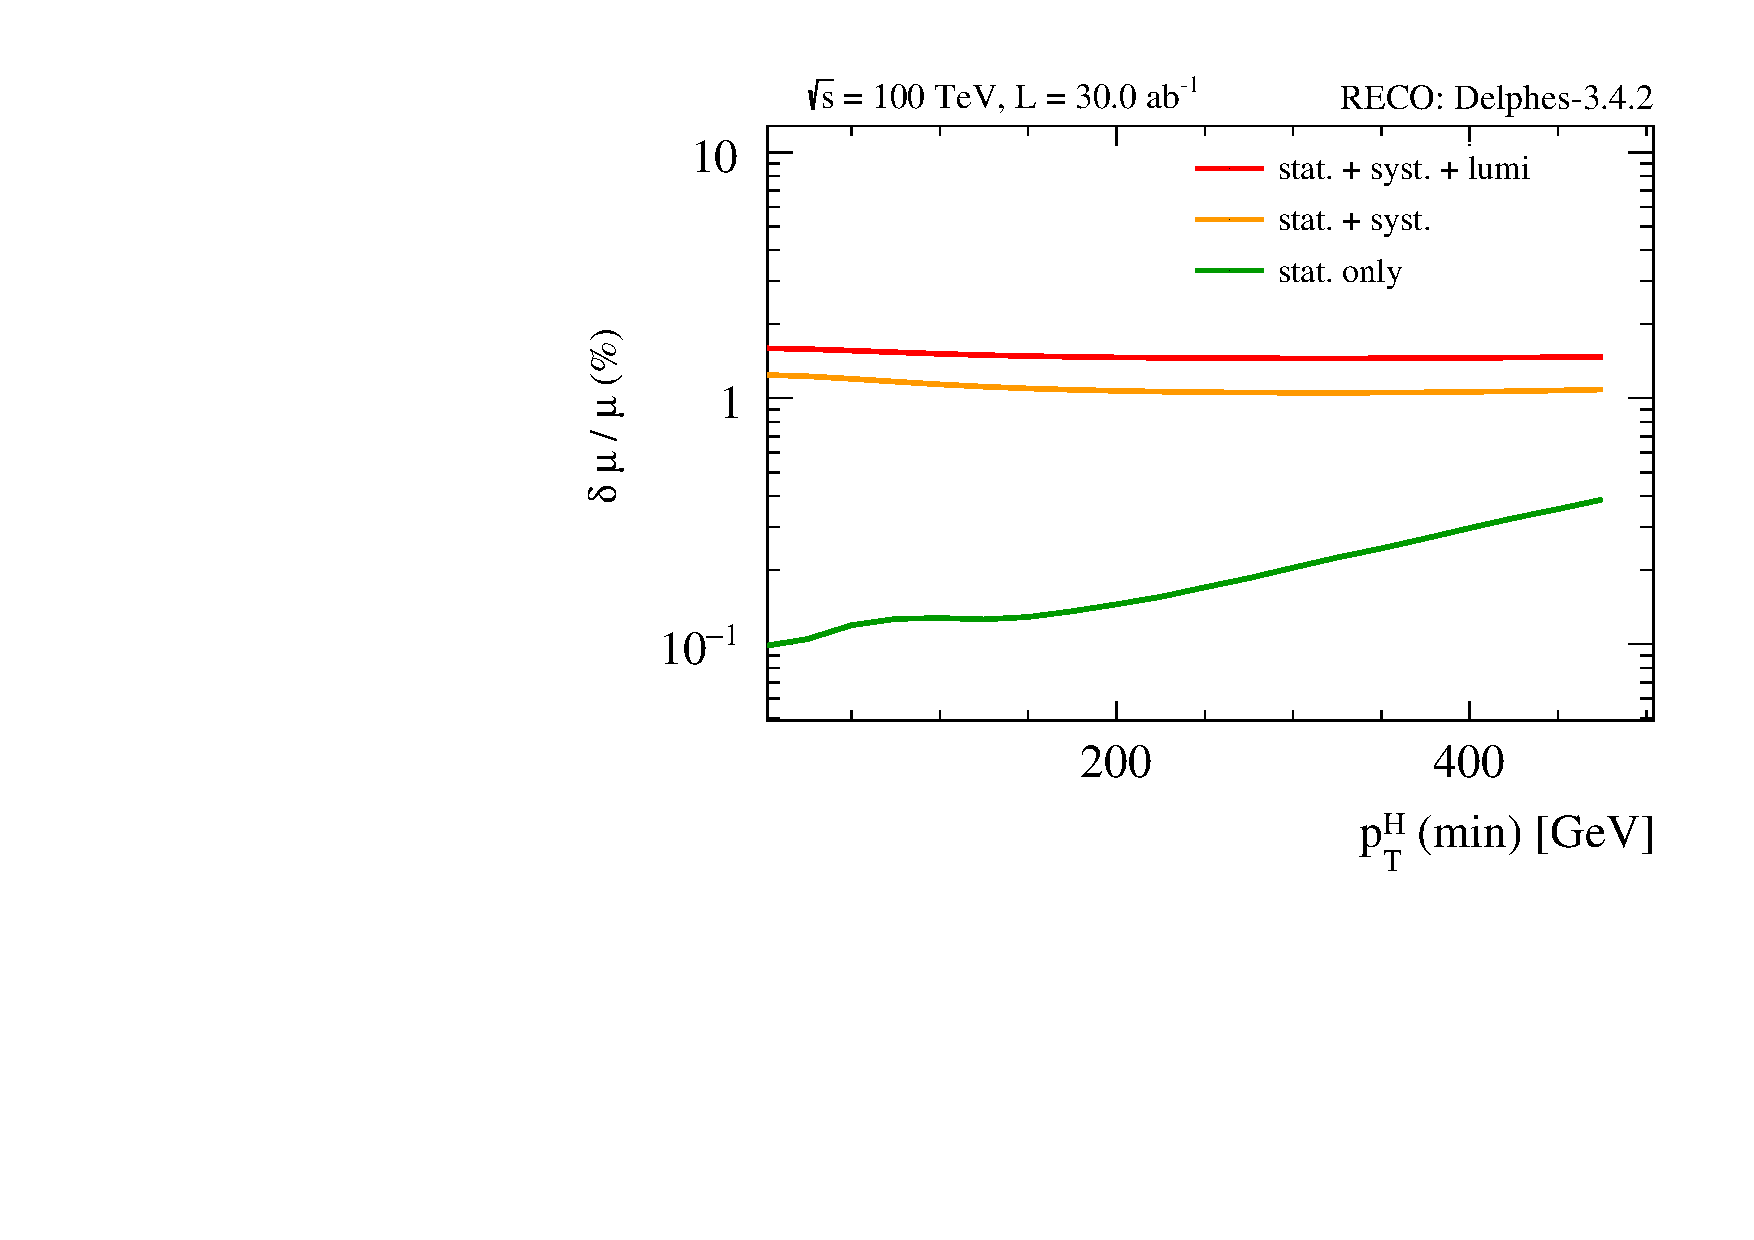
\includegraphics[width=0.45\textwidth]{\main/Neutrino/img/hgg.pdf} .
%\end{verbatim}

%\begin{figure}[ht]
%\centering
%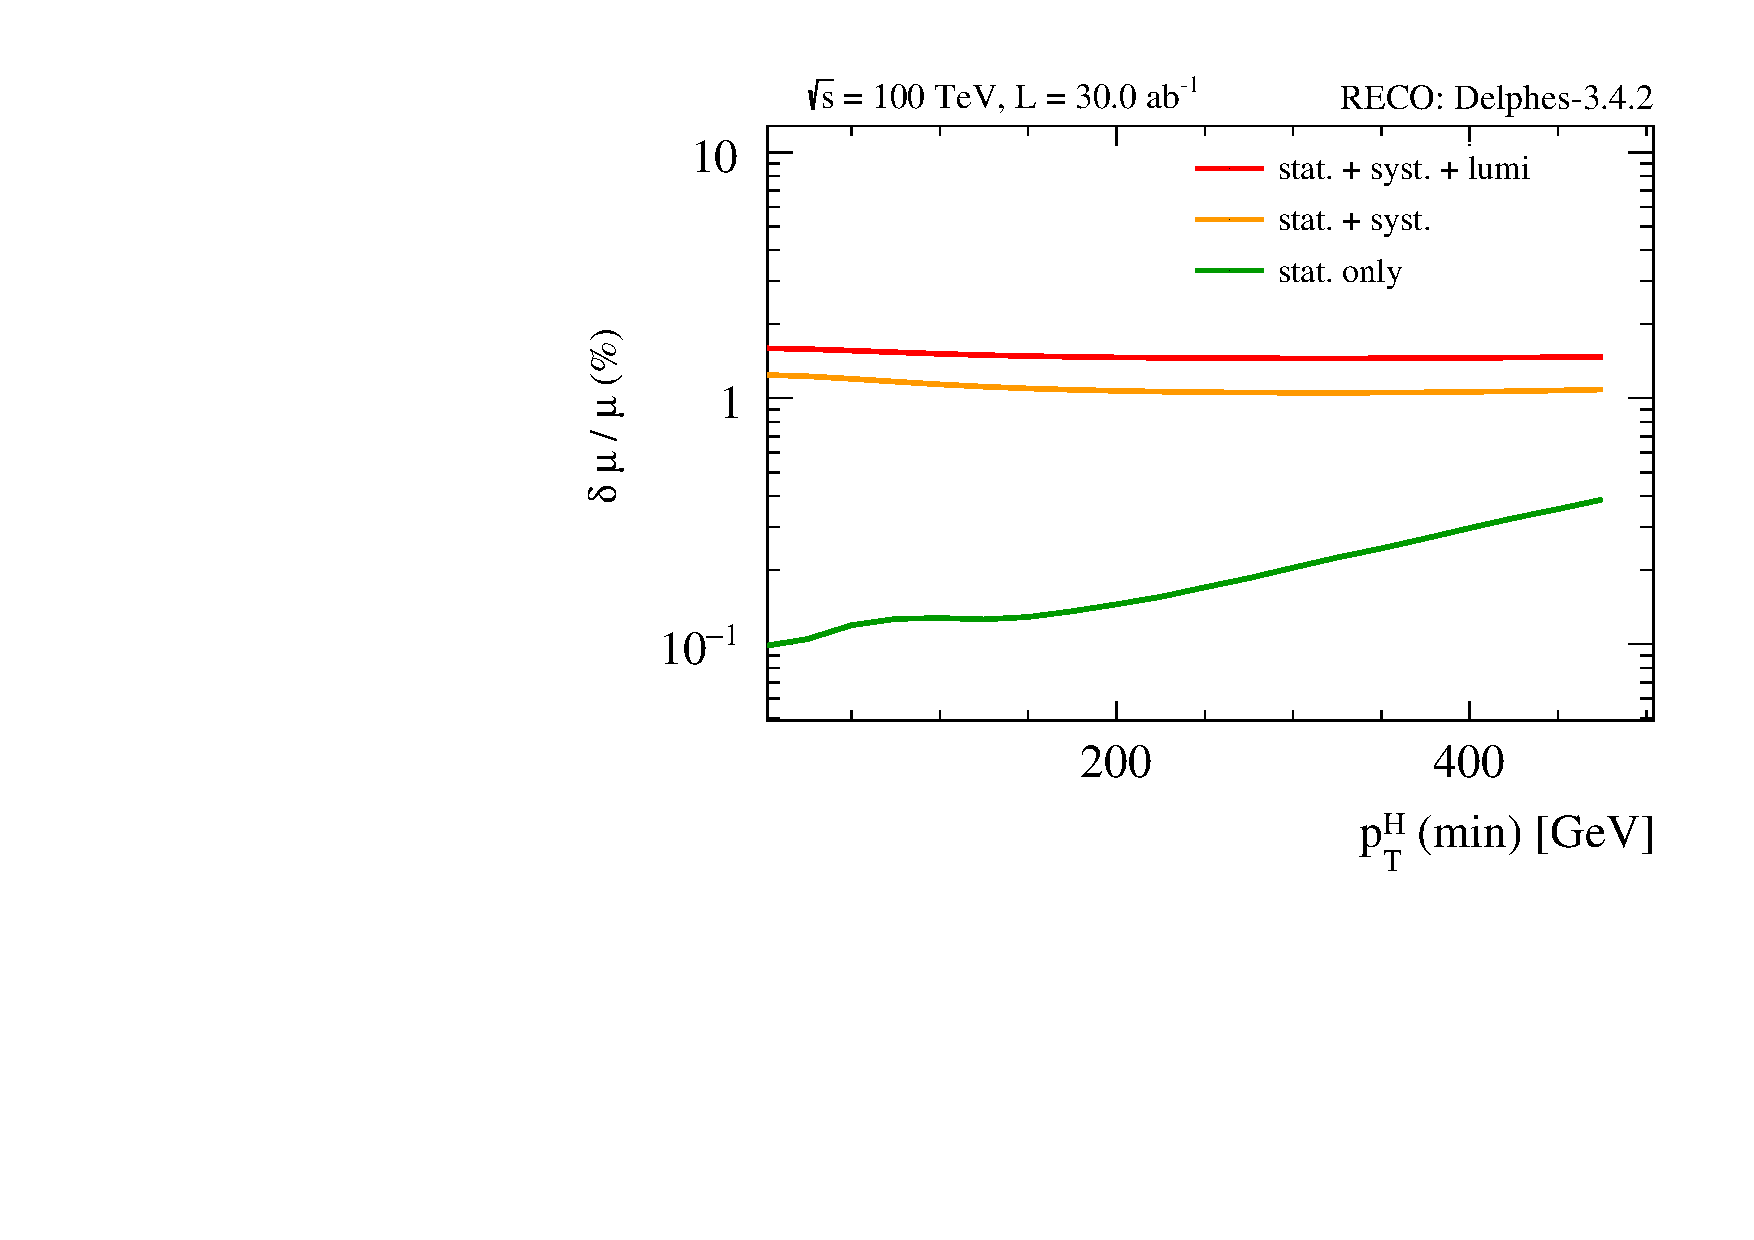
\includegraphics[width=0.75\textwidth]{\main/Neutrino/img/hgg.pdf}
%\caption{Caption of the figure.}
%\label{fig:higgs}
%\end{figure}

%As for tables, please use the standard tabular environment, with the
%caption on top of the table. For cross referencing, try use lables
%such as
%\verb|\label{eq:eqname}|, \verb|\label{tab:tabname}| and
%\verb|\label{fig:figname}|. 


%\subfile{\main/Neutrino/sub1/mysubsec}


\end{document}

